\documentclass{article}
\usepackage{tikz}
\usepackage{listings}

\begin{document}
% This works fine, too. But it's global.
\lstset{
  language=TeX,
  %keywordstyle=\color{blue}\ttfamily,
  %numberstyle=\ttfamily,
  %stringstyle=\ttfamily,
  basicstyle=\ttfamily,
}
\noindent
\begin{lstlisting}[
  basicstyle=\small\ttfamily,
]
  \textbackslash{}begin{tikzpicture}
    \textbackslash{}filldraw [gray] (0,0) circle [radius=2pt]
                     (1,1) circle [radius=2pt]
                     (2,1) circle [radius=2pt]
                     (2,0) circle [radius=2pt];
    \textbackslash{}draw (0,0) .. controls (1,1) and (2,1) .. (2,0);
  \textbackslash{}end{tikzpicture}
\end{lstlisting}

\vspace{1em}
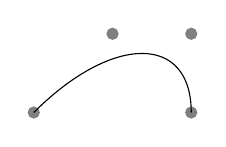
\begin{tikzpicture}
  \filldraw [gray] (0,0) circle [radius=2pt]
                   (1,1) circle [radius=2pt]
                   (2,1) circle [radius=2pt]
                   (2,0) circle [radius=2pt];
  \draw (0,0) .. controls (1,1) and (2,1) .. (2,0);
\end{tikzpicture}


\noindent \rule{\paperwidth}{1pt}
\vspace{2em}


\noindent
\begin{lstlisting}
  \textbackslash{}begin{tikzpicture}
    \textbackslash{}filldraw [gray] (0,0) circle [radius=2pt]
                     (1,1) circle [radius=2pt]
                     (2,1) circle [radius=2pt]
                     (2,0) circle [radius=2pt];
    \textbackslash{}draw (0,0) .. controls (1,1) .. (2,0);
  \textbackslash{}end{tikzpicture}
\end{lstlisting}
\vspace{3em}
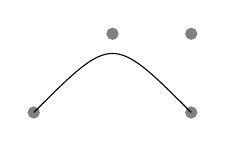
\begin{tikzpicture}
  \filldraw [gray] (0,0) circle [radius=2pt]
                   (1,1) circle [radius=2pt]
                   (2,1) circle [radius=2pt]
                   (2,0) circle [radius=2pt];
  \draw (0,0) .. controls (1,1) .. (2,0);
\end{tikzpicture}


\noindent \rule{\paperwidth}{1pt}
\vspace{2em}


\noindent
\begin{lstlisting}
  \textbackslash{}begin{tikzpicture}
    \textbackslash{}filldraw [gray] (0,0) circle [radius=2pt]
                     (1,1) circle [radius=2pt]
                     (2,1) circle [radius=2pt]
                     (2,0) circle [radius=2pt];
    \textbackslash{}draw (0,0) .. controls (1,1) and (1,1) .. (2,0);
  \textbackslash{}end{tikzpicture}
\end{lstlisting}
\vspace{2em}
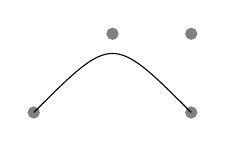
\begin{tikzpicture}
  \filldraw [gray] (0,0) circle [radius=2pt]
                   (1,1) circle [radius=2pt]
                   (2,1) circle [radius=2pt]
                   (2,0) circle [radius=2pt];
  \draw (0,0) .. controls (1,1) and (1,1) .. (2,0);
\end{tikzpicture}

\end{document}
